% ______________________________________________________________________________
%
%   2DV513 Database Theory -- Assignment 1
%
%   Author:  Jonas Sjöberg
%            Linnaeus University
%            js224eh@student.lnu.se
%            github.com/jonasjberg
%            www.jonasjberg.com
%
%  License:  Creative Commons Attribution 4.0 International (CC BY 4.0)
%            <http://creativecommons.org/licenses/by/4.0/legalcode>
%            See LICENSE.md for additional licensing information.
% ______________________________________________________________________________


\section{Task 3 --- The Registrars Office}
Exercise from \emph{Database System Concepts, 5th Edition} \cite{2dv513:dsc},
section 6.2.

\subsection{Problem Description}
The problem description \cite{2dv513:assignment1-instructions} is stated as
follows:

\begin{quote}
  A university registrar's office maintains data about the following entities:

  \begin{enumerate}
    \item
      (a) courses, include number, title, credits, syllabus, and prerequisites;

    \item
      (b) course offerings, include course number, year, semester, section
      number, instructor(s), timings, and classroom;
  
    \item
      (c) students, including student-id, name, and program; and
  
    \item
      (d) instructors, including identification number, name, department, and
      title.
  \end{enumerate}

  Further, the enrollment of students in courses and grades awarded to students
  in each course they are enrolled for must be appropriately modeled.
  
  Construct an E/R diagram for the registrar's office.
\end{quote}


\subsection{Solution}
The propsed solution is shown in Figure~\ref{fig:task3}.

\begin{figure}[htbp]
  \centering
  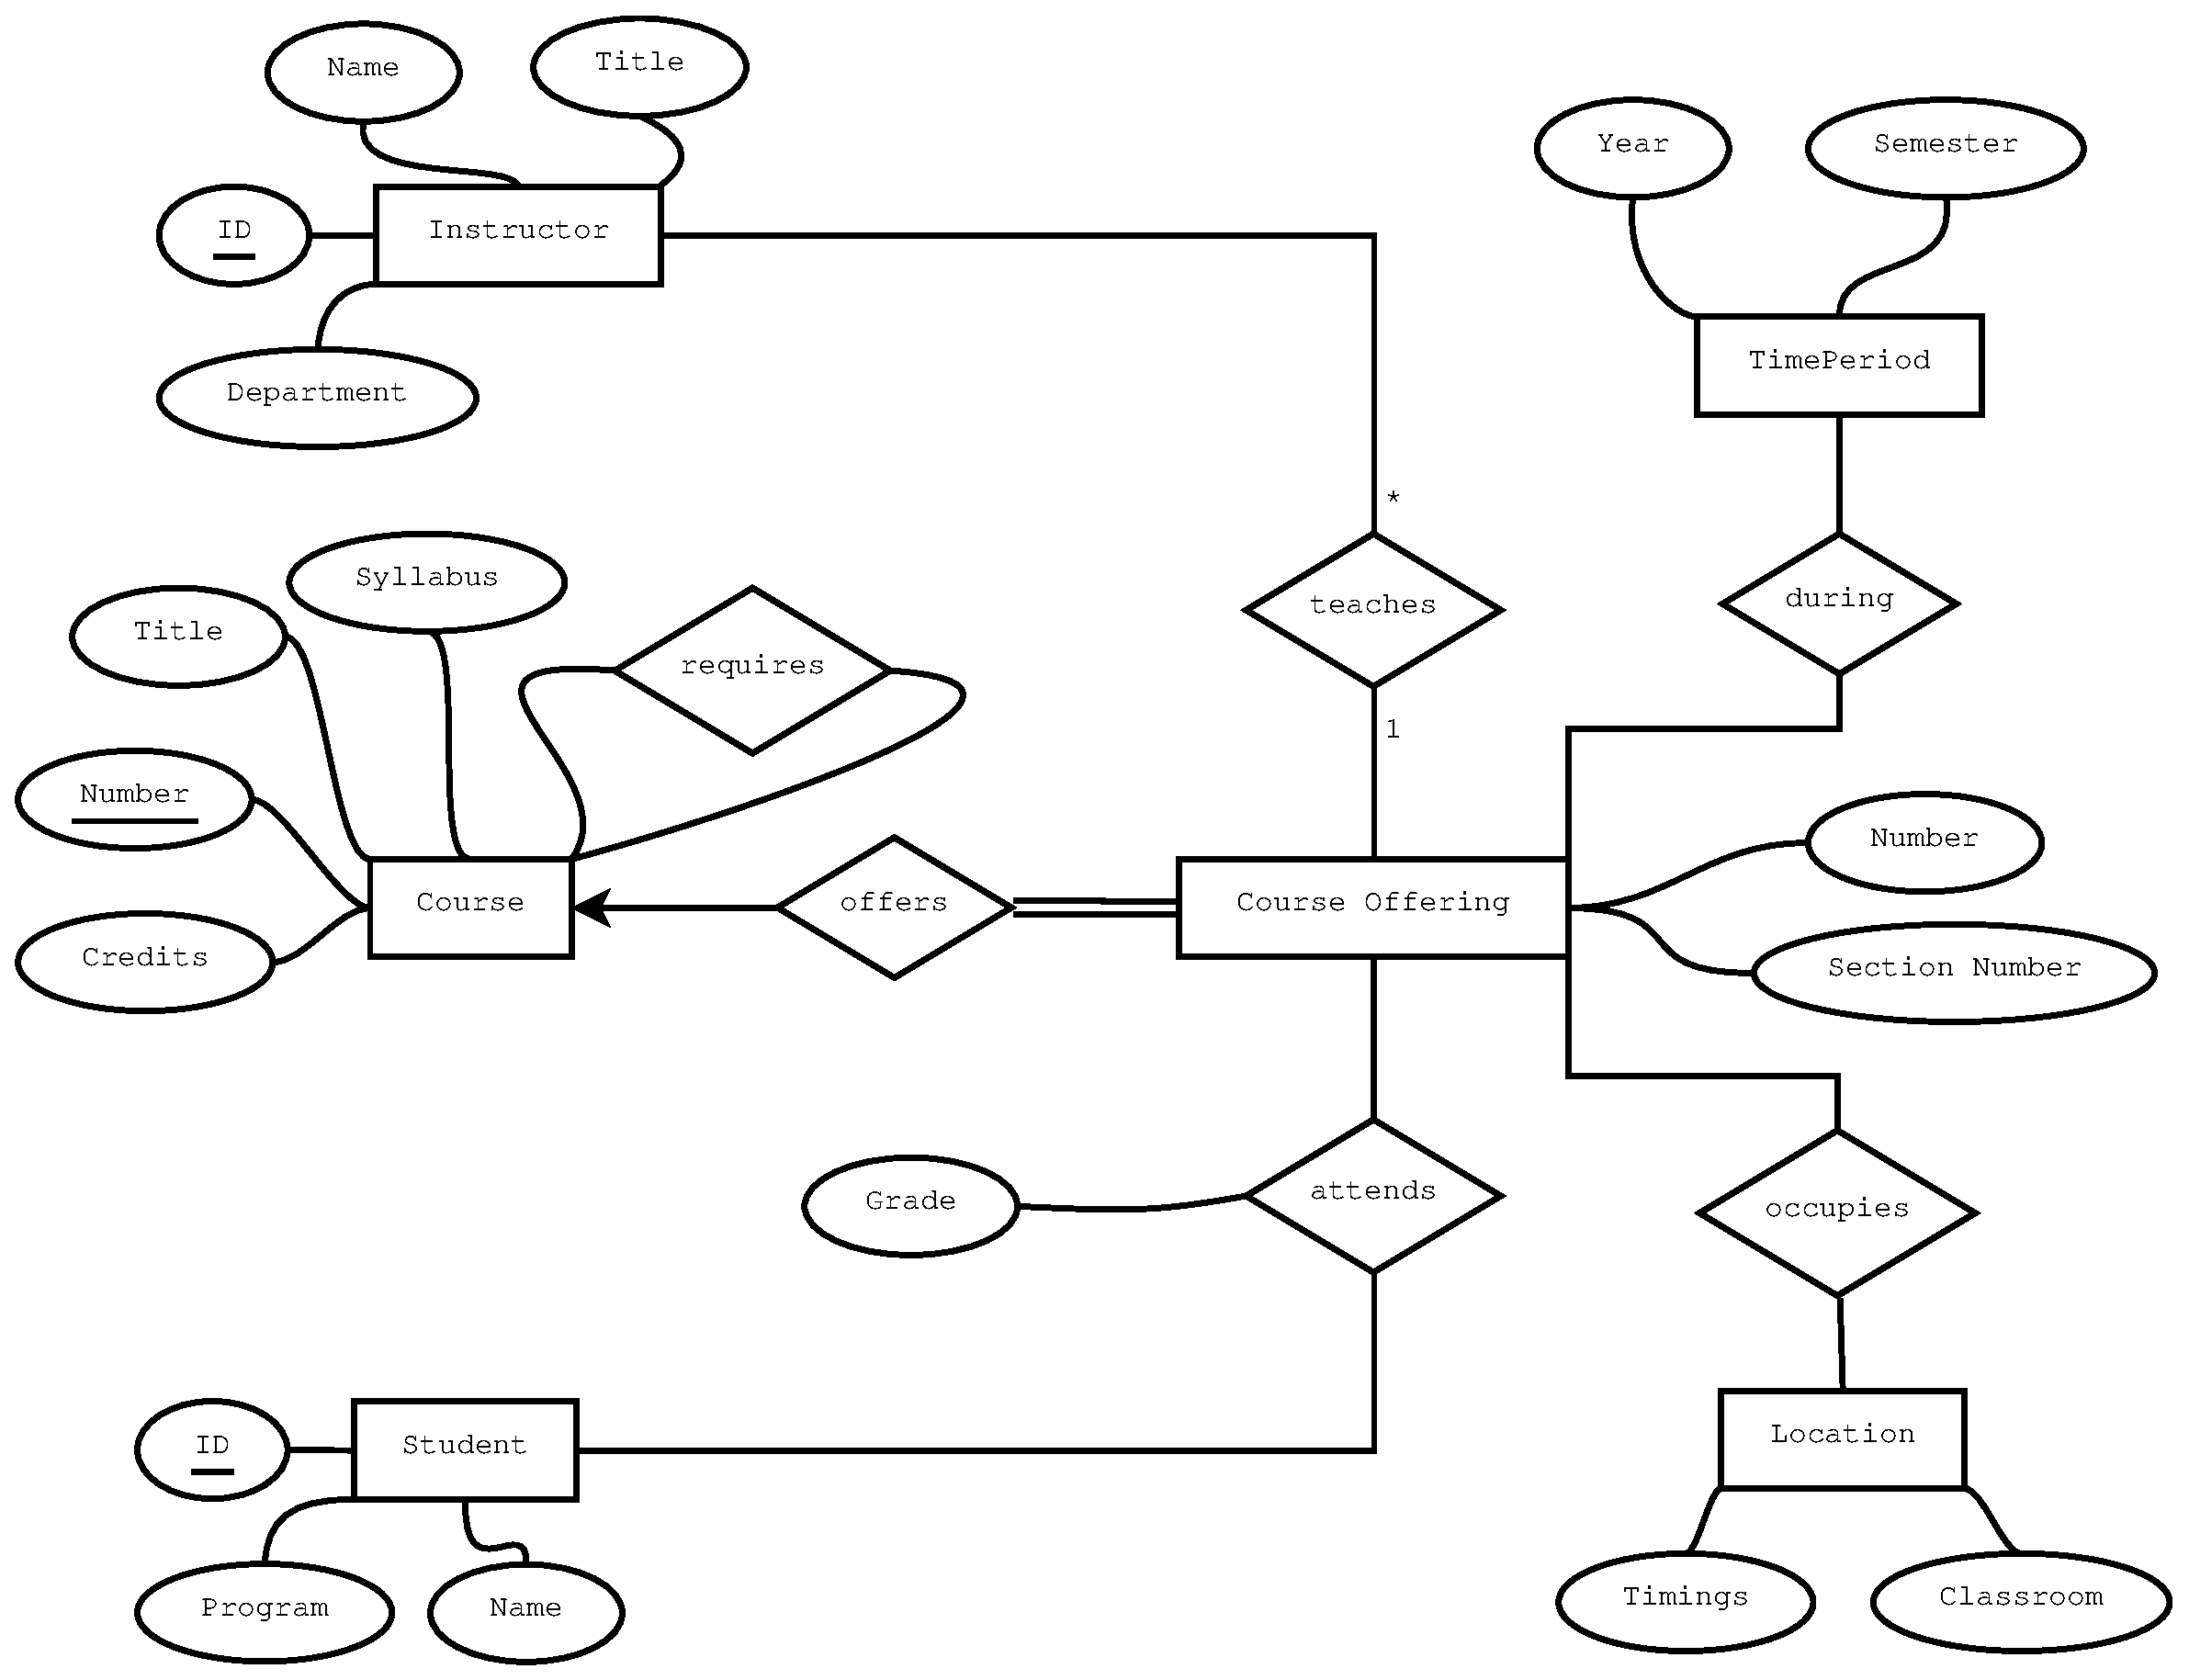
\includegraphics[width=\linewidth]{include/task3.eps}
    \caption{Entity-relationship Diagram for Task 3}
  \label{fig:task3}
\end{figure}

Some of the attributes have been bundled into new entities.
